\documentclass[12pt,a4paper]{article}

% ─── Page Layout ───────────────────────────────────────────────────────────────
\usepackage[a4paper, margin=0.8in, headheight=14pt]{geometry}

% ─── Fonts (XeLaTeX) ───────────────────────────────────────────────────────────
\usepackage{fontspec}
\usepackage{unicode-math}
\setmainfont{TeX Gyre Pagella}
\setmonofont[Scale=0.88]{TeX Gyre Cursor}
\setmathfont{Latin Modern Math}

% ─── Packages ──────────────────────────────────────────────────────────────────
\usepackage{xcolor}
\usepackage{colortbl}
\usepackage{titlesec}
\usepackage{enumitem}
\usepackage{tabularx}
\usepackage{booktabs}
\usepackage{array}
\usepackage{amsmath}
\usepackage{tikz}
\usetikzlibrary{shapes.geometric, arrows.meta, positioning, calc, fit, decorations.pathreplacing}
\usepackage{tcolorbox}
\tcbuselibrary{skins, breakable}
\usepackage{hyperref}
\usepackage{fancyhdr}
\usepackage{graphicx}
\usepackage{microtype}
\hyphenpenalty=10000
\exhyphenpenalty=10000
\sloppy
\usepackage{caption}
\usepackage{setspace}
\usepackage{multirow}
\usepackage{tocloft}

% ─── Q&A helper ────────────────────────────────────────────────────────────────
\newcommand{\Q}[1]{\textbf{#1}\par\noindent\ignorespaces}

% ─── Colour Palette ────────────────────────────────────────────────────────────
\definecolor{myred}{RGB}{196,30,58}
\definecolor{mydark}{RGB}{30,30,50}
\definecolor{mygreen}{RGB}{14,120,80}
\definecolor{myteal}{RGB}{0,130,140}
\definecolor{myamber}{RGB}{180,100,0}
\definecolor{mypurple}{RGB}{100,30,160}
\definecolor{mygray}{RGB}{246,247,249}
\definecolor{mgframe}{RGB}{180,185,200}
\definecolor{watermark}{RGB}{145,150,170}
\definecolor{hdrred}{RGB}{250,232,235}
\definecolor{hdrgreen}{RGB}{220,244,233}
\definecolor{hdrteal}{RGB}{220,242,244}
\definecolor{hdramber}{RGB}{253,242,215}
\definecolor{hdrpurple}{RGB}{238,228,255}
\definecolor{hdrgray}{RGB}{238,240,245}
\definecolor{rowalt}{RGB}{250,251,253}

% ─── Section Formatting ────────────────────────────────────────────────────────
\titleformat{\section}
  {\large\bfseries\color{myred}}{\thesection.}{0.5em}{}
  [\vspace{1pt}{\color{myred}\rule{\linewidth}{0.8pt}}]
\titleformat{\subsection}
  {\normalsize\bfseries\color{myteal}}{\thesubsection}{0.5em}{}
\titlespacing*{\section}{0pt}{18pt}{7pt}
\titlespacing*{\subsection}{0pt}{11pt}{4pt}

% ─── Paragraph ─────────────────────────────────────────────────────────────────
\setlength{\parindent}{0pt}
\setlength{\parskip}{4pt}

% ─── TOC Styling ───────────────────────────────────────────────────────────────
\renewcommand{\cfttoctitlefont}{\large\bfseries\color{myred}}
\renewcommand{\cftaftertoctitle}{\par\noindent{\color{myred}\rule{\linewidth}{0.8pt}}}
\setlength{\cftbeforetoctitleskip}{0pt}
\setlength{\cftaftertoctitleskip}{6pt}
\renewcommand{\cftsecfont}{\normalsize\bfseries\color{mydark}}
\renewcommand{\cftsecpagefont}{\normalsize\bfseries\color{mydark}}
\renewcommand{\cftsecleader}{\cftdotfill{\cftdotsep}}
\setlength{\cftbeforesecskip}{7pt}
\renewcommand{\cftsubsecfont}{\small\color{mydark}}
\renewcommand{\cftsubsecpagefont}{\small\color{mydark}}
\setlength{\cftbeforesubsecskip}{3pt}
\setlength{\cftsubsecindent}{1.4em}

% ─── Table helpers ─────────────────────────────────────────────────────────────
\renewcommand{\arraystretch}{1.45}
\setlength{\tabcolsep}{6pt}
\arrayrulecolor{mydark}
\newcolumntype{B}[1]{>{\small\bfseries\raggedright\arraybackslash}m{#1}}
\newcolumntype{Y}{>{\small\raggedright\arraybackslash}X}
\renewcommand{\tabularxcolumn}[1]{m{#1}}

% ─── Header / Footer ───────────────────────────────────────────────────────────
\pagestyle{fancy}
\fancyhf{}
\fancyhead[L]{\small\color{myred}\textbf{OE-EC604C}\;\color{mydark}--- Object Oriented Programming}
\fancyhead[R]{\small\color{myteal}\textbf{Module 8 Notes}}
\fancyfoot[C]{\small\color{mydark}\thepage}
\fancyfoot[R]{\small\color{watermark}\textit{\copyright\ Biraj}}
\renewcommand{\headrulewidth}{0.5pt}
\renewcommand{\footrulewidth}{0.3pt}

% ─── Hyperref ──────────────────────────────────────────────────────────────────
\hypersetup{
  colorlinks=true, linkcolor=myteal, urlcolor=myteal,
  pdfauthor={Biraj Sarkar},
  pdftitle={OE-EC604C --- Module 8 Notes}
}

% ─── tcolorbox styles ──────────────────────────────────────────────────────────
\tcbset{
  tikzbox/.style={
    colback=mygray, colframe=mgframe, boxrule=0.6pt, arc=4pt,
    left=8pt, right=8pt, top=6pt, bottom=6pt,
    colbacktitle=mgframe, coltitle=mydark,
    fonttitle=\small\bfseries
  },
  defbox/.style={
    colback=hdrgreen, colframe=mygreen, boxrule=0.8pt, arc=4pt,
    left=9pt, right=9pt, top=6pt, bottom=6pt,
    colbacktitle=mygreen, coltitle=white,
    fonttitle=\small\bfseries
  },
  formulabox/.style={
    colback=hdrteal, colframe=myteal, boxrule=0.8pt, arc=4pt,
    left=9pt, right=9pt, top=7pt, bottom=7pt,
    colbacktitle=myteal, coltitle=white,
    fonttitle=\small\bfseries
  },
  examplebox/.style={
    colback=hdramber, colframe=myamber, boxrule=0.8pt, arc=4pt,
    left=9pt, right=9pt, top=6pt, bottom=6pt,
    colbacktitle=myamber, coltitle=white,
    fonttitle=\small\bfseries
  },
  masonbox/.style={
    colback=hdrpurple, colframe=mypurple, boxrule=0.8pt, arc=4pt,
    left=9pt, right=9pt, top=6pt, bottom=6pt,
    colbacktitle=mypurple, coltitle=white,
    fonttitle=\small\bfseries
  },
  exambox/.style={
    colback=hdrpurple, colframe=mypurple, boxrule=1pt, arc=5pt,
    left=10pt, right=10pt, top=8pt, bottom=8pt,
    colbacktitle=mypurple, coltitle=white,
    fonttitle=\bfseries,
    breakable, title after break={\textbf{Frequently Asked / Viva Questions (contd.)}}}
}
% Make all boxes breakable across pages
\tcbset{breakable}

% ─── TikZ styles ───────────────────────────────────────────────────────────────
\tikzset{
  block/.style={rectangle, draw=myteal, fill=hdrteal,
    text width=2.4cm, align=center, minimum height=0.95cm,
    font=\small, rounded corners=3pt, line width=0.7pt},
  redblock/.style={rectangle, draw=myred, fill=hdrred,
    text width=2.4cm, align=center, minimum height=0.95cm,
    font=\small, rounded corners=3pt, line width=0.7pt},
  netnode/.style={rectangle, draw=myteal, fill=hdrteal,
    text width=1.5cm, align=center, minimum height=0.8cm,
    font=\small, rounded corners=3pt, line width=0.7pt},
  sumjunc/.style={circle, draw=myamber, fill=hdramber,
    minimum size=0.62cm, font=\small, line width=0.8pt},
  snode/.style={circle, draw=mypurple, fill=hdrpurple,
    minimum size=0.55cm, font=\footnotesize, line width=0.7pt},
  arrow/.style={-Stealth, thick, color=mydark},
  redarrow/.style={-Stealth, thick, color=myred},
  line/.style={thick, color=mydark}
}

% ═══════════════════════════════════════════════════════════════════════════════
\begin{document}
% ═══════════════════════════════════════════════════════════════════════════════

\begin{center}
  {\LARGE\bfseries\color{myred} OE-EC604C --- Object Oriented Programming}\\[5pt]
  {\normalsize\color{mydark} Semester VI \quad$\bullet$\quad 3L:0T:0P \quad$\bullet$\quad 3 Credits}\\[3pt]
  {\normalsize\color{myteal}\textbf{Module 8 Exam Notes: Files and Streams}}\\[3pt]
  {\small\color{mydark} CGEC \;$|$\; B.Tech ECE (2023--27) \;$|$\; \textit{Biraj Sarkar}}
\end{center}
\vspace{2pt}
\noindent{\color{myred}\rule{\linewidth}{1.5pt}}
\vspace{2pt}

\hypersetup{linkcolor=mydark}
\tableofcontents
\hypersetup{linkcolor=myteal}
\newpage

% ===============================================================================
\section{C++ File Streams Hierarchy}
% ===============================================================================

C++ models file input and output operations using a system of classes inherited from basic stream classes.

\subsection{The Stream Class Hierarchy}
All stream classes are derived from a common virtual base class \texttt{ios}. The main classes used for file operations are:
\begin{itemize}[leftmargin=*, itemsep=3.5pt]
  \item \textbf{\texttt{ifstream}:} Input file stream. Derived from \texttt{istream}, used for reading files.
  \item \textbf{\texttt{ofstream}:} Output file stream. Derived from \texttt{ostream}, used for creating and writing files.
  \item \textbf{\texttt{fstream}:} Input/Output file stream. Derived from \texttt{iostream}, used for simultaneous reading and writing operations.
\end{itemize}

\begin{tcolorbox}[tikzbox, title={C++ Stream Class Hierarchy Topology}]
\centering
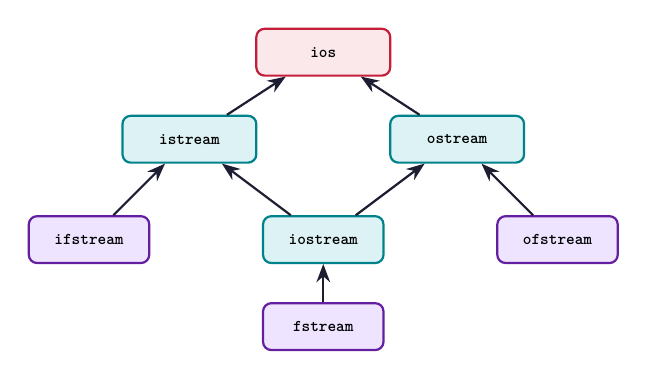
\begin{tikzpicture}[node distance=1.2cm, thick, scale=0.85, every node/.style={scale=0.85}]
  % Root node
  \node[rectangle, draw=myred, fill=hdrred, rounded corners=3pt, minimum width=2.0cm, minimum height=0.7cm, font=\scriptsize\bfseries] (ios) at (0, 2.0) {\texttt{ios}};

  % Intermediate nodes
  \node[rectangle, draw=myteal, fill=hdrteal, rounded corners=3pt, minimum width=2.0cm, minimum height=0.7cm, font=\scriptsize\bfseries] (istream) at (-2.0, 0.7) {\texttt{istream}};
  \node[rectangle, draw=myteal, fill=hdrteal, rounded corners=3pt, minimum width=2.0cm, minimum height=0.7cm, font=\scriptsize\bfseries] (ostream) at (2.0, 0.7) {\texttt{ostream}};

  % Derived stream classes
  \node[rectangle, draw=mypurple, fill=hdrpurple, rounded corners=3pt, minimum width=1.8cm, minimum height=0.7cm, font=\scriptsize\bfseries] (ifstream) at (-3.5, -0.8) {\texttt{ifstream}};
  \node[rectangle, draw=myteal, fill=hdrteal, rounded corners=3pt, minimum width=1.8cm, minimum height=0.7cm, font=\scriptsize\bfseries] (iostream) at (0, -0.8) {\texttt{iostream}};
  \node[rectangle, draw=mypurple, fill=hdrpurple, rounded corners=3pt, minimum width=1.8cm, minimum height=0.7cm, font=\scriptsize\bfseries] (ofstream) at (3.5, -0.8) {\texttt{ofstream}};

  % Bottom fstream node
  \node[rectangle, draw=mypurple, fill=hdrpurple, rounded corners=3pt, minimum width=1.8cm, minimum height=0.7cm, font=\scriptsize\bfseries] (fstream) at (0, -2.1) {\texttt{fstream}};

  % Inheritance arrows
  \draw[arrow] (istream) -- (ios);
  \draw[arrow] (ostream) -- (ios);
  \draw[arrow] (ifstream) -- (istream);
  \draw[arrow] (iostream) -- (istream);
  \draw[arrow] (iostream) -- (ostream);
  \draw[arrow] (ofstream) -- (ostream);
  \draw[arrow] (fstream) -- (iostream);
\end{tikzpicture}
\tcbset{colbacktitle=mgframe, coltitle=mydark}
\end{tcolorbox}

% ===============================================================================
\section{Opening \& Closing Files}
% ===============================================================================

Files can be opened in two ways: using the constructor or using the \texttt{open()} method.

\subsection{File Open Methods}
\begin{enumerate}[label=\textbf{\arabic*.}, leftmargin=*, itemsep=3pt]
  \item \textbf{Using Constructor:} Best when managing a single file throughout the stream's lifetime.
    \begin{equation}
      \texttt{ofstream outFile("data.txt"); // Opens file automatically}
    \end{equation}
  \item \textbf{Using \texttt{open()} method:} Best when reusing a single stream object to access multiple files sequentially.
    \begin{equation}
      \texttt{ifstream inFile; inFile.open("data.txt");}
    \end{equation}
\end{enumerate}

\subsection{File Modes}
File modes specify the access permissions and options for opening files.
\renewcommand{\arraystretch}{1.3}
\par\noindent
\begin{tabularx}{\linewidth}{|B{3.4cm}|Y|}
\hline
\textbf{File Mode Constant} & \textbf{Description} \\
\hline
\texttt{ios::in} & Opens the file for reading (default for \texttt{ifstream}). \\
\hline
\texttt{ios::out} & Opens the file for writing (default for \texttt{ofstream}). Erases existing content. \\
\hline
\texttt{ios::app} & Append mode. All write operations occur at the end of the file. \\
\hline
\texttt{ios::ate} & Opens the file and moves the pointer to the end of the file. \\
\hline
\texttt{ios::binary} & Opens the file in binary mode (instead of default text mode). \\
\hline
\end{tabularx}

% ===============================================================================
\section{File Pointers and Seek Operations}
% ===============================================================================

Each file stream object maintains file pointers that keep track of reading or writing locations.

\subsection{Seek and Tell Functions}
\begin{itemize}[leftmargin=*, itemsep=3.5pt]
  \item \textbf{\texttt{seekg()}:} Moves the \textbf{get} (read) pointer to a new position.
  \item \textbf{\texttt{seekp()}:} Moves the \textbf{put} (write) pointer to a new position.
  \item \textbf{\texttt{tellg()}:} Returns the current offset position of the get pointer.
  \item \textbf{\texttt{tellp()}:} Returns the current offset position of the put pointer.
\end{itemize}

\begin{tcolorbox}[defbox, title={\textbf{Seek Syntax Parameters}}]
\begin{align}
  &\texttt{stream.seekg(offset, direction);} \\
  &\text{Where direction can be: } \texttt{ios::beg} \quad \text{or} \quad \texttt{ios::cur} \quad \text{or} \quad \texttt{ios::end}
\end{align}
\end{tcolorbox}

\begin{tcolorbox}[tikzbox, title={File Pointer Position and Offset Directions}]
\centering
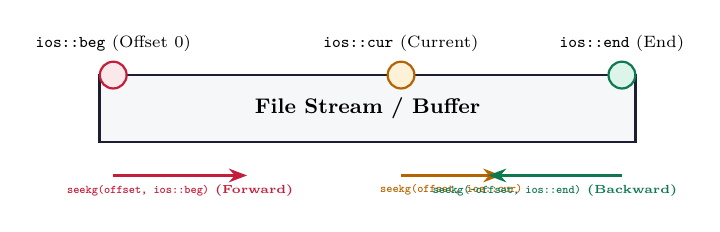
\begin{tikzpicture}[node distance=1.5cm, thick, scale=0.85, every node/.style={scale=0.85}]
  % File Buffer box
  \draw[draw=mydark, fill=mygray, line width=1.0pt] (-4.0, 0.5) rectangle (4.0, -0.5);
  \node[font=\small\bfseries] at (0, 0) {File Stream / Buffer};

  % Anchor Points
  \node[circle, draw=myred, fill=hdrred, minimum size=0.4cm, label=above:{\scriptsize\texttt{ios::beg} (Offset 0)}] (beg) at (-3.8, 0.5) {};
  \node[circle, draw=myamber, fill=hdramber, minimum size=0.4cm, label=above:{\scriptsize\texttt{ios::cur} (Current)}] (cur) at (0.5, 0.5) {};
  \node[circle, draw=mygreen, fill=hdrgreen, minimum size=0.4cm, label=above:{\scriptsize\texttt{ios::end} (End)}] (end) at (3.8, 0.5) {};

  % Seek Operations
  \draw[arrow, color=myred] (-3.8, -1.0) -- (-1.8, -1.0) node[midway, below, font=\tiny\bfseries] {\texttt{seekg(offset, ios::beg)} (Forward)};
  \draw[arrow, color=myamber] (0.5, -1.0) -- (2.0, -1.0) node[midway, below, font=\tiny\bfseries] {\texttt{seekg(offset, ios::cur)}};
  \draw[arrow, color=mygreen] (3.8, -1.0) -- (1.8, -1.0) node[midway, below, font=\tiny\bfseries] {\texttt{seekg(-offset, ios::end)} (Backward)};
\end{tikzpicture}
\tcbset{colbacktitle=mgframe, coltitle=mydark}
\end{tcolorbox}

% ===============================================================================
\section{Binary \& Random Access Operations}
% ===============================================================================

By default, files are opened in text mode. Binary mode allows reading and writing complete structures or objects to files directly without parsing.

\subsection{Object Writing using \texttt{write()} and \texttt{read()}}
\begin{align}
  &\texttt{file.write(reinterpret\_cast<char*>(\&object), sizeof(object));} \\
  &\texttt{file.read(reinterpret\_cast<char*>(\&object), sizeof(object));}
\end{align}

\begin{tcolorbox}[examplebox, title={Code Example: Reading and writing objects to binary files}]
\begin{spacing}{1.0}
\begin{verbatim}
#include <iostream>
#include <fstream>
#include <cstring>
class Student {
private:
    char name[30];
    int roll;
public:
    Student() : roll(0) { name[0] = '\0'; }
    Student(const char* n, int r) {
        strcpy(name, n);
        roll = r;
    }
    void show() {
        std::cout << "Roll: " << roll << ", Name: " << name << std::endl;
    }
};

void saveRecord() {
    Student s1("Biraj", 101);
    std::ofstream file("student.dat", std::ios::out | std::ios::binary);
    file.write(reinterpret_cast<char*>(&s1), sizeof(s1));
    file.close();
}

void loadRecord() {
    Student s2;
    std::ifstream file("student.dat", std::ios::in | std::ios::binary);
    file.read(reinterpret_cast<char*>(&s2), sizeof(s2));
    s2.show(); // Prints: Roll: 101, Name: Biraj
    file.close();
}
\end{verbatim}
\end{spacing}
\tcbset{colbacktitle=myamber, coltitle=white}
\end{tcolorbox}

\subsection{Random Access Database Record Update}
Using \texttt{seekp()} and index logic, we can update specific object slots directly inside a binary database without reading the whole file.

\begin{tcolorbox}[examplebox, title={Code Example: Random Access database record update}]
\begin{spacing}{1.0}
\begin{verbatim}
#include <iostream>
#include <fstream>
struct Account {
    int accNum;
    double balance;
};

void updateBalance(int recordId, double newBalance) {
    std::fstream file("account.dat", std::ios::in | std::ios::out | std::ios::binary);
    Account acc;
    
    // Jump to the specific record offset using sizeof
    int offset = (recordId - 1) * sizeof(Account);
    file.seekp(offset, std::ios::beg);
    
    acc.accNum = recordId;
    acc.balance = newBalance;
    
    // Rewrite record
    file.write(reinterpret_cast<char*>(&acc), sizeof(Account));
    file.close();
}
\end{verbatim}
\end{spacing}
\tcbset{colbacktitle=myamber, coltitle=white}
\end{tcolorbox}

% ===============================================================================
% MANDATORY QUICK REVISION PAGE
% ===============================================================================
\newpage
\begin{center}
  {\large\bfseries\color{myred} Quick Revision --- Module VIII}\\[3pt]
  {\small\color{mydark} Files and Streams $|$ OE-EC604C}
\end{center}
\noindent{\color{myred}\rule{\linewidth}{1.2pt}}
\vspace{4pt}

\begin{tcolorbox}[formulabox, title={\textbf{Key File I/O Syntax}}]
\renewcommand{\arraystretch}{1.3}
\begin{tabularx}{\linewidth}{B{3.8cm} X}
Open Write (Trunc)       & \texttt{ofstream out("a.txt", ios::out); // overrides} \\[4pt]
Open Append              & \texttt{ofstream out("a.txt", ios::app); // appends} \\[4pt]
Binary Open              & \texttt{fstream file("a.dat", ios::in | ios::out | ios::binary);} \\[4pt]
Seek from Beginning      & \texttt{file.seekg(100, ios::beg); // jumps to offset 100} \\[4pt]
Seek Backward (End)      & \texttt{file.seekp(-50, ios::end); // jumps 50 bytes before EOF} \\[4pt]
Get Current Position     & \texttt{int pos = file.tellg(); // returns read offset}
\end{tabularx}
\end{tcolorbox}

\begin{tcolorbox}[defbox, title={\textbf{One-Line Definitions}}]
\begin{itemize}[leftmargin=*, itemsep=2.5pt, topsep=0pt]
  \item \textbf{File Stream:} The logical interface that connects the program to physical files on the disk.
  \item \textbf{ifstream:} A file stream class specialized in reading data from disk files.
  \item \textbf{ofstream:} A file stream class specialized in writing data to disk files.
  \item \textbf{fstream:} A stream class that supports both input and output file operations.
  \item \textbf{File Mode:} Settings that configure file permissions (read, write, binary, append) when a file is opened.
  \item \textbf{Get Pointer:} The read pointer that keeps track of the next index byte to read from a file.
  \item \textbf{Put Pointer:} The write pointer that keeps track of the next index byte to write to a file.
  \item \textbf{tellg():} A file function returning the current index offset of the read (get) pointer.
  \item \textbf{seekg():} A file function used to reposition the get pointer to a specified index location.
  \item \textbf{Binary Mode:} Opening a file to write raw memory bytes directly, bypassing text formatting.
\end{itemize}
\end{tcolorbox}

\begin{tcolorbox}[exambox, title={\textbf{Frequently Asked / Viva Questions}}]
\begin{enumerate}[topsep=0pt, label=\textbf{Q\arabic*.}, itemsep=5pt]
  \item \Q{What is the difference between opening a file using constructor vs. the \texttt{open()} method?}
    The constructor automatically opens the file and is clean for single files. The `open()` function allows opening multiple files sequentially using the same stream object.
  \item \Q{Explain the difference between the \texttt{ios::app} and \texttt{ios::ate} file modes.}
    Both open the file with pointers positioned at the end. However, `ios::app` forces all write operations to occur at the end of the file, whereas `ios::ate` allows shifting the pointer to write anywhere in the file.
  \item \Q{Why is \texttt{reinterpret\_cast<char*>} mandatory in \texttt{read()} and \texttt{write()} functions?}
    These functions are designed to accept a stream of bytes (`char*`). We must cast our class object address to a byte pointer for binary transfer.
  \item \Q{What is random file access and how is it implemented in C++?}
    Random access allows reading/writing at any arbitrary location in the file without processing it sequentially. It is implemented using `seekg()`, `seekp()`, `tellg()`, and `tellp()`.
  \item \Q{What happens if we attempt to open a non-existent file for reading?}
    The file stream fails to open, and its error flag is set. We can verify this state using the `fail()` function or checking the stream's truth value: `if(!file)`.
  \item \Q{Why must we close files explicitly before exiting the program?}
    Closing files flushes the stream buffers (saving unwritten data from RAM to disk) and releases system file handles.
  \item \Q{Can we open a single file for simultaneous reading and writing?}
    Yes, using the `fstream` class and combining file modes: `fstream file("data.dat", ios::in | ios::out | ios::binary)`.
  \item \Q{What is the purpose of the \texttt{eof()} function in C++ streams?}
    It returns `true` if the get pointer has reached the end-of-file (EOF) during a read operation.
  \item \Q{How does text mode file access differ from binary mode file access?}
    Text mode translates line endings (like converting \texttt{\textbackslash n} to \texttt{\textbackslash r\textbackslash n} on Windows) and parses values. Binary mode copies raw memory bytes bit-by-bit without any translations.
  \item \Q{Which class acts as the root class for all file stream classes?}
    The root class is `ios` (specifically, \texttt{ios\_base} is the grandparent class, and `ios` inherits from it).
  \item \Q{How can we determine the total size of a file in bytes using seek functions?}
    We can seek to the end of the file and use `tellg()` to query the pointer offset:
    `file.seekg(0, ios::end); int size = file.tellg();`.
  \item \Q{What is a file stream buffer and why is it used?}
    It is a temporary block of memory in RAM that buffers read/write bytes to minimize slow disk access operations, improving performance.
\end{enumerate}
\tcbset{colbacktitle=mypurple, coltitle=white}
\end{tcolorbox}

\begin{tcolorbox}[tikzbox, title={Comparison: Sequential File Access vs. Random File Access}]
\renewcommand{\arraystretch}{1.45}
\par\noindent
\begin{tabularx}{\linewidth}{|B{3.2cm}|Y|Y|}
\hline
\textbf{Feature} & \textbf{\color{myteal}Sequential File Access} & \textbf{\color{myamber}Random File Access} \\
\hline
\textbf{Pointer Mechanics} & Pointers move step-by-step from beginning to end. & Pointers can jump directly to any arbitrary offset. \\
\hline
\textbf{Speed} & Slower for large databases (must read intermediate records). & Extremely fast (access time is constant, $O(1)$, using offsets). \\
\hline
\textbf{File Functions} & Uses standard operators like \texttt{<<}, \texttt{>>}, or getline. & Uses functions like \texttt{seekg()}, \texttt{seekp()}, \texttt{tellg()}, \texttt{tellp()}. \\
\hline
\textbf{Common Modes} & Text mode (comma/space-separated values). & Binary mode (fixed-size struct or class records). \\
\hline
\textbf{Use Case} & Reading configuration files or writing log lines. & Modifying specific records in a large binary database. \\
\hline
\end{tabularx}
\tcbset{colbacktitle=mgframe, coltitle=mydark}
\end{tcolorbox}

\end{document}
